\section{Обработка табличных данных. Часть 2}
\subsection{Условие задания}
Выполнить задание. Вариант: <<Заменить столбцы, содержащие только чётные элементы, столбцом X.>>.

Создать приложение для выполнения задания. Использовать элемент формы DataGridView. Диапазон $[a,b]$ означает, что $mas[i][j] >= a$ и $mas[i][j] <= b$

Приложение должно выполнять следующие действия:

\begin{enumerate}
\item Возможность удалять и добавлять строки таблицы. Проект не должен аварийно завершаться при удалении несуществующей таблицы.
\item Проверять ввод не числовых данных как в таблицу, так и в остальные текстовые поля (если есть в задании).
\item Если есть диапазон значений $[a,b]$, проверять, что $a < b$.
\item Заголовок формы должен отражать суть задания.
\item Все элементы формы должны быть внятно подписаны (кнопки подписаны, у тестового поля должно быть написано, для чего оно нужно и т. д.)
\item В коде должны быть комментарии и отступы (код должен быть легко читаем).
\item В коде программы все элементы формы должны быть переименованы (btnName -  для кнопок, lblName - для ссылок, txtName - для текстового поля и т.д.) Наименования должны быть понятными.
\item Приложение должно корректно работать (выводить ответ или ошибку с соответствующим сообщением). После вывода ошибок при вводе корректных данных поля ошибок должны очищаться.  
\end{enumerate}

\subsection{Вид формы в конструкторе}
Форма имеет вид:

\begin{figure}
\centering
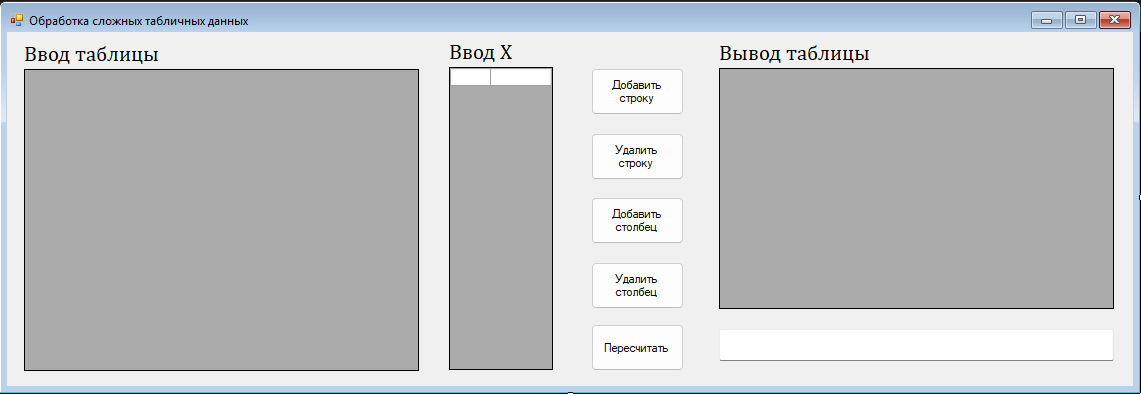
\includegraphics[width=0.5\linewidth]{images/handling-data-hard/form.png}
\caption{Форма окна для задания <<Простые вычисления>>}
\label{handling-data-hard-form}
\end{figure}

\subsection{Таблица с описанием элементов формы}
Все элементы формы были переименованы для большей читаемости. В таблице \ref{tab:handling-data-hard-form} представлены все изменения.

\begin{table}
\centering
\begin{tabular}{|m{0.3\textwidth}|m{0.3\textwidth}|m{0.3\textwidth}|}
\hline
\textbf{Описание элементов формы} & \textbf{Список изменённых атрибутов} & \textbf{Новое значение атрибута} \\
\hline
\hline
Окно формы & Text & Обработка сложных табличных данных \\
Метка <<Ввод таблицы>> & Name & tableInputLabel \\
Метка <<Ввод X>> & Name & xInputLabel \\
Метка <<Вывод таблицы>> & Name & outputLabel \\
Основная таблица ввода & Name & tableGrid \\
Дополнительная таблица ввода & Name & xGrid \\
Таблица вывода & Name & outputGridView \\
Поле для ошибок & Name & errorProvider \\
Кнопка <<Добавить строку>> & Name & addRow \\
Кнопка <<Удалить строку>> & Name & removeRow \\
Кнопка <<Добавить столбец>> & Name & addColumn \\
Кнопка <<Удалить столбец>> & Name & removeColumn \\
Кнопка <<Пересчитать>> & Name & executeButton \\

\hline
\end{tabular}
\caption{Значение атрибутов элементов в приложении для обработки табличных данных}
\label{tab:handling-data-hard-form}
\end{table}

\subsection{Примеры правильной и неправильной работы приложения}
При запуске приложения на экране появляется окно \ref{fig:handling-data-hard-start}.

\begin{figure}
\centering
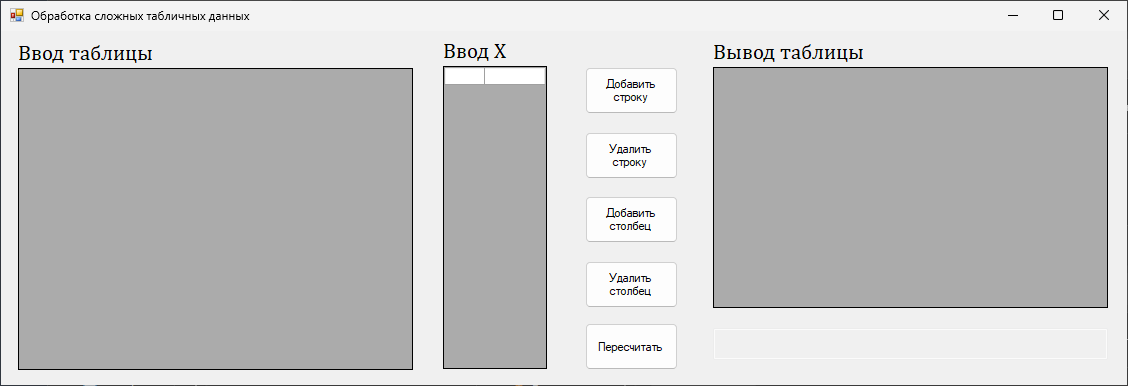
\includegraphics[width=0.5\linewidth]{images//handling-data-hard/start.png}
\caption{Запуск программы}
\label{fig:handling-data-hard-start}
\end{figure}

При нажатии на кнопку подсчитываются и подставляются значения в таблицу вывода. Также происходит обработка ошибок.

\begin{figure}
\centering
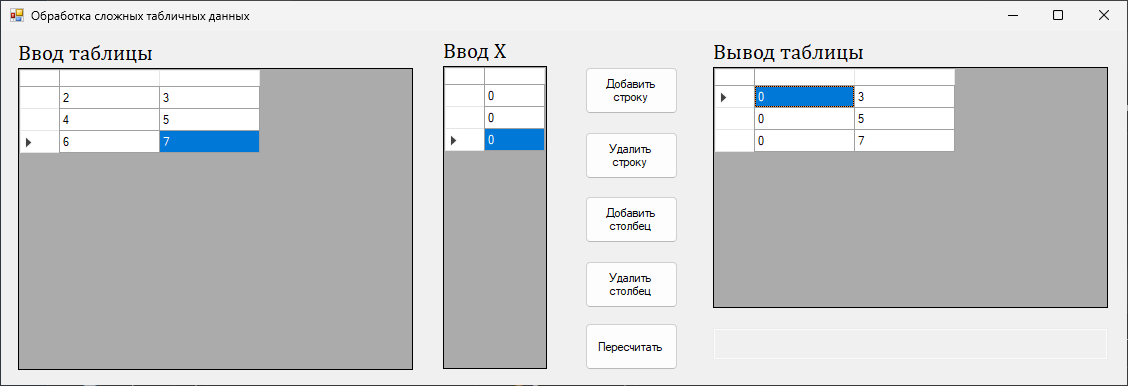
\includegraphics[width=0.5\linewidth]{images//handling-data-hard/okay.png}
\caption{Запуск с корректными данными}
\label{fig:handling-data-hard-okay}
\end{figure}

\begin{figure}
\centering
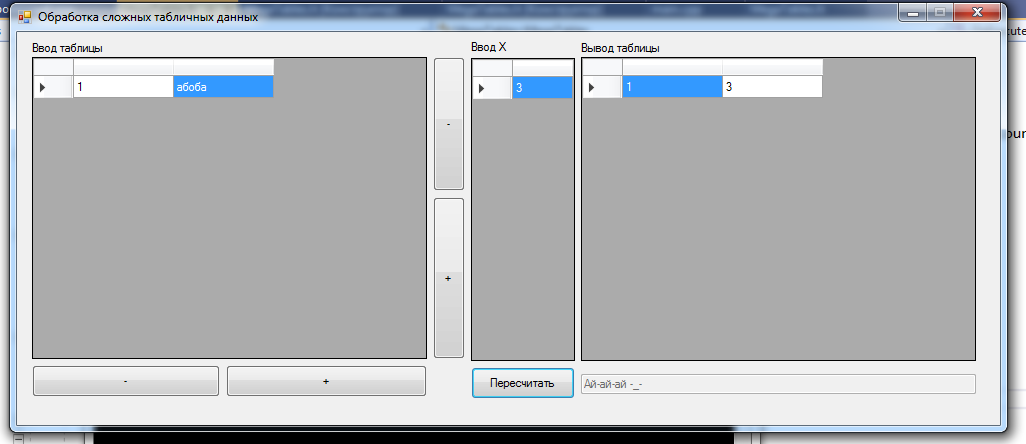
\includegraphics[width=0.5\linewidth]{images//handling-data-hard/error.png}
\caption{Пример ввода с некорректными данными}
\label{fig:handling-data-hard-error}
\end{figure}

\begin{figure}
\centering
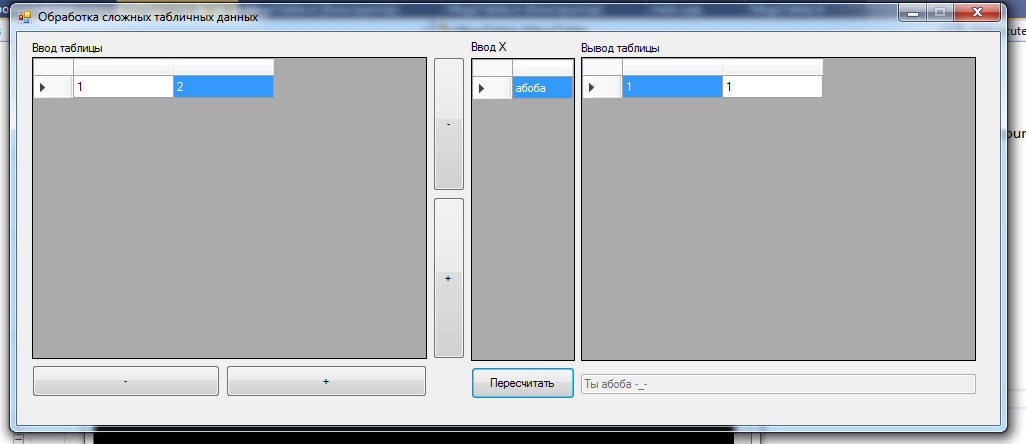
\includegraphics[width=0.5\linewidth]{images//handling-data-hard/error2.png}
\caption{Пример ввода с некорректными данными}
\label{fig:handling-data-hard-error2}
\end{figure}

\subsection{Примеры исходного кода}
\begin{minted}{cpp}
/* функция для обсчёта массива данных */
private: System::Void executeButton_Click(System::Object^ sender, System::EventArgs^ e) {
    int evenColumns = 0;
    try {
        for (int j = 0; j < this->tableGrid->Columns->Count; ++j) {
            bool flag = true;
            for (int i = 0; i < this->tableGrid->Rows->Count; ++i) {
                int value;
                Int32::TryParse(System::Convert::ToString(this->tableGrid->Rows[tableGrid->RowCount - i - 1]->Cells[j]->Value), value);
                if (value % 2 != 0) {
                    flag = false;
                    break;
                }
            }
    
            evenColumns++;
            for (int i = 0; i < this->tableGrid->Rows->Count; ++i) {
                if (flag) {
                    this->outputGridView->Rows[tableGrid->RowCount - i - 1]->Cells[j]->Value = this->xGrid->Rows[tableGrid->RowCount - i - 1]->Cells[0]->Value;
                }
                else {
                    this->outputGridView->Rows[tableGrid->RowCount - i - 1]->Cells[j]->Value = this->tableGrid->Rows[tableGrid->RowCount - i - 1]->Cells[j]->Value;
                }
    
            }
        }
    
        if (!evenColumns) {
            this->errorProvider->Text = "Нет чётных столбцов";
        }
    }
    catch (...) {
        this->errorProvider->Text = "Не удалось заменить столбцы";
    }
}
\end{minted}

Больше кода проекта доступно в приложении \ref{application-A}. Также в приложенном архиве можно найти полный код проекта.